\documentclass[12pt]{article}

% Packages


% Packages
\usepackage{graphicx}
\usepackage{setspace}
\usepackage{geometry}
\usepackage{natbib}
\usepackage{hyperref}
\hypersetup{hidelinks}
\usepackage{parskip}
\usepackage{float}
\usepackage{tikz}
\usetikzlibrary{positioning,arrows.meta}
\usepackage{float}

% Page setup
\geometry{margin=1in}
\onehalfspacing

% Title details
\title{
    \vspace{-2cm}
    \textbf{Factors Associated with Life Satisfaction Among Women in Canada}\\
    \vspace{0.4cm}
    \large An Analysis of Socioeconomic, Employment, and Health-Related Determinants\\
    \large Using Canadian Community Health Survey (CCHS 2022) Data
}

\author{
    Khushboo Singh\\
    \vspace{0.3cm}
    MSc Data Science and Analytics\\
    Toronto Metropolitan University\\
    \vspace{0.3cm}
    Supervisor: Dr. Ozgur Turetken
}

\date{July 2026}

\begin{document}

\maketitle

\begin{abstract}

Life satisfaction is an important indicator of subjective well-being and reflects how individuals evaluate their overall quality of life. This study examined demographic, socioeconomic, employment-related, and health-related factors associated with low life satisfaction among women in Canada using data from the 2022 Canadian Community Health Survey (CCHS) Public Use Microdata File.

The exploratory analysis included 52,884 women. Life satisfaction was first examined using its original five-category measure. For predictive modeling, respondents who reported being Dissatisfied or Very Dissatisfied were classified as having low life satisfaction. After additional data-cleaning steps, the final modeling sample contained 52,543 respondents, of whom approximately 6.31\% were classified as having low life satisfaction.

Descriptive analysis, visualizations, Chi-square tests, and Cramer's V were used to examine relationships between life satisfaction and selected predictors. The exploratory findings showed that food security and functional difficulty had the strongest associations with low life satisfaction. Household income and labour force status also showed meaningful relationships, while education and province had weaker associations.

The predictive modeling stage compared a majority-class baseline with Logistic Regression, Decision Tree, Random Forest, and Gradient Boosting models. Class weighting, hyperparameter tuning, cross-validation, and validation-based threshold selection were used to address the imbalanced outcome. All substantive models identified more low-life-satisfaction cases than the baseline. Gradient Boosting achieved the highest held-out PR-AUC of 0.204, although its improvement over Random Forest and Logistic Regression was small. Functional difficulty, food security, and labour force status were the most consistently important predictors across the models.

Overall, the results suggest that material conditions and health-related functioning are important factors associated with low life satisfaction among women in the analytical sample. The findings represent associations and predictive patterns rather than causal relationships.Since the analyses were based on unweighted data, the results should
not be interpreted as nationally representative estimates for all
women in Canada.

\end{abstract}

\section{Introduction}

Life satisfaction is an important indicator of subjective well-being and overall quality of life. It reflects how individuals evaluate their life as a whole, rather than only measuring the presence or absence of illness \citep{diener1984, kahneman2010}. For this reason, life satisfaction is commonly used in public health, social science, and population health research to understand broader well-being.

This study focuses on the relationship between objective living conditions and subjective well-being. Subjective well-being refers to how individuals evaluate and experience their own lives, while objective well-being refers to measurable conditions such as income, employment, food security, education, and health status. Although life satisfaction is a subjective measure, it can be influenced by these objective conditions because they affect access to resources, daily activities, independence, and overall quality of life \citep{diener1984, kahneman2010}.

Women's well-being may be influenced by several demographic, socioeconomic, employment-related, and health-related factors. Previous research has shown that women's health and well-being are shaped by social and economic conditions, work and family responsibilities, caregiving roles, income, social support, and health status \citep{denton2004, matud2014, bilodeau2025}. These factors may affect how women experience their daily lives and how they evaluate their overall life satisfaction.

Socioeconomic conditions are also important for understanding life satisfaction. Income, education, food security, and employment status have been linked to differences in subjective well-being across populations \citep{kahneman2010, clark1994, tarasuk2023}. Individuals with greater financial security and access to resources are generally more likely to report higher life satisfaction, while those experiencing financial hardship, unemployment, or material deprivation may report lower well-being.

Health-related factors are another important part of life satisfaction. Functional limitations, chronic health conditions, and difficulties with everyday activities may affect independence, employment participation, social participation, and quality of life. Prior research has identified health status as an important factor associated with subjective well-being and life satisfaction \citep{diener1984, denton2004}.

The post-pandemic context also makes this topic relevant. The COVID-19 pandemic affected employment, caregiving responsibilities, financial security, and social conditions for many Canadians, and these effects may continue to influence well-being \citep{park2024, bilodeau2025}. Studying life satisfaction using recent Canadian survey data can therefore help identify factors associated with women's well-being after the pandemic period.

Although previous studies have examined different determinants of well-being, many focus on specific factors such as income, employment, or health separately. Fewer studies examine demographic, socioeconomic, employment-related, and health-related variables together using recent Canadian population-level data. There is also a need for interpretable analytical approaches that can show which factors are most strongly associated with lower life satisfaction.

Based on these gaps, this study addresses two main research questions. First, which demographic, socioeconomic, employment-related, and health-related factors are associated with low life satisfaction among women in Canada? Second, how well can these variables identify women with low life satisfaction, and which predictors appear consistently important across different classification models?

This study used data from the 2022 Canadian Community Health Survey to examine factors associated with low life satisfaction among women in Canada. The analysis combined exploratory data analysis, statistical testing, and predictive modeling. Logistic Regression and Decision Tree Classification were included as relatively interpretable methods, while Random Forest and Gradient Boosting were used to examine whether more flexible ensemble approaches improved predictive performance. By comparing findings across descriptive, statistical, and predictive methods, the study aimed to identify factors that consistently appeared important and to contribute to a better understanding of women's subjective well-being in the Canadian post-pandemic context.



\section{Literature Review}

\subsection{Life Satisfaction and Subjective Well-Being}

Life satisfaction is an important component of subjective well-being. It refers to how individuals evaluate their life as a whole, rather than only measuring a specific emotional state or clinical mental health condition. Unlike clinical measures of depression, anxiety, or psychological disorder, life satisfaction captures a broader evaluation of quality of life. For this reason, it is commonly used in population-level studies of well-being \citep{diener1984, diener1999}.

\citet{diener1984} described subjective well-being as a broad concept that includes life satisfaction, positive affect, and negative affect. Later research also emphasized that life satisfaction is a useful measure because it reflects an individual's overall judgment of life circumstances, rather than only short-term emotions \citep{diener1999, diener2013}. This distinction is important because well-being is not only about the absence of illness, but also about how people evaluate their lives and experiences.

Life satisfaction is also useful for connecting subjective well-being with objective living conditions. Although life satisfaction is based on an individual's own evaluation, it can be influenced by measurable factors such as income, employment, health, food security, education, and social conditions. For example, previous research has shown that income is more strongly related to life evaluation than to some measures of emotional well-being \citep{kahneman2010}. This suggests that life satisfaction is an appropriate outcome for studying how broader socioeconomic and health-related conditions are associated with well-being.

This distinction is important for the current study because the 2022 Canadian Community Health Survey does not provide a suitable clinical mental health outcome for the full analytical sample used in this project. However, it does include a life satisfaction variable, which provides a meaningful measure of subjective well-being. Using life satisfaction as the outcome allows this study to examine how demographic, socioeconomic, employment-related, and health-related factors are associated with well-being among women in Canada.

Overall, the literature suggests that life satisfaction is shaped by multiple factors, including income, employment, health, social support, and personal circumstances \citep{diener1984, diener1999, diener2013, kahneman2010}. Therefore, examining life satisfaction among women requires attention to broader determinants such as financial security, food security, employment participation, functional health, and social context.

\subsection{Women and Life Satisfaction}

Women’s life satisfaction may be influenced by several social, economic, health-related, and gender-related factors. Previous research has shown that women’s health and well-being are connected to employment conditions, income, caregiving responsibilities, household roles, social support, and chronic stress exposure \citep{denton2004, matud2014, artazcoz2004, bilodeau2025}. These factors can affect daily life, quality of life, and overall well-being.

\citet{denton2004} examined gender differences in health in Canada and found that health outcomes are influenced by psychosocial, structural, and behavioural determinants. Their study showed that women’s health and well-being are affected by employment conditions, income, caregiving responsibilities, and chronic stress exposure. These findings are relevant to the current study because they support the idea that women’s well-being should be examined within a broader social determinants framework rather than through individual characteristics alone.

Gender roles and social relationships may also influence life satisfaction. \citet{matud2014} examined life satisfaction among adult women and men and found that self-esteem and social support were among the strongest predictors of life satisfaction. Their study also showed that social support played an important role in women’s life satisfaction. This suggests that women’s subjective well-being may be shaped not only by economic and health conditions, but also by social relationships and psychosocial resources.

Research on work-family dynamics further supports the importance of gendered experiences in well-being. \citet{bilodeau2025} found that women often experience greater work-family conflict and emotional strain due to unequal caregiving and domestic responsibilities. Similarly, \citet{artazcoz2004} showed that combining paid work and family demands affects men and women differently, with women often experiencing greater health-related consequences when managing both employment and caregiving responsibilities.

Overall, existing literature suggests that women’s life satisfaction is influenced by multiple overlapping factors, including socioeconomic status, employment conditions, caregiving responsibilities, health, and social support. These findings support the need for a women-focused analysis of life satisfaction using recent Canadian population-level data.

\subsection{Socioeconomic Factors and Life Satisfaction}
\subsubsection{Income and Life Satisfaction}

Income has been linked to life satisfaction because it affects access to material resources, housing, food, transportation, and other necessities \citep{kahneman2010}. Financial security may also reduce stress and provide individuals with greater control over their life circumstances. For this reason, income is commonly considered an important socioeconomic factor in studies of subjective well-being.

\citet{kahneman2010} distinguished between emotional well-being and life evaluation. Their study found that income was more strongly associated with life evaluation than with day-to-day emotional well-being. They argued that higher income improves how individuals evaluate their lives overall, even though emotional well-being may not continue to improve beyond a certain income level. This distinction is directly relevant to the current study because life satisfaction is closer to life evaluation than to a clinical measure of mental health.

The relationship between income and life satisfaction is important for understanding well-being among women in Canada. Women with lower household income may experience greater financial strain, difficulty meeting household needs, housing insecurity, and reduced access to resources. These pressures may contribute to lower overall life satisfaction. Therefore, household income is included in this study as a key socioeconomic predictor.

\subsubsection{Food Security and Life Satisfaction}

Food security is another important socioeconomic factor related to well-being. Household food insecurity refers to inadequate or insecure access to food because of financial constraints, and it reflects broader material deprivation and economic hardship \citep{tarasuk2023}. For this reason, food insecurity is not only a food-related issue, but also an indicator of socioeconomic vulnerability.

\citet{tarasuk2023} reported that household food insecurity in Canada reached a record high in 2022, with 17.8\% of households in the ten provinces experiencing some level of food insecurity. The report emphasized that food insecurity is strongly linked to low income, limited assets, debt, and other forms of socioeconomic disadvantage. It also identified food insecurity as a major social determinant of health, associated with poorer physical and mental health, greater healthcare use, hospitalization, and premature mortality.

Food insecurity is particularly relevant to women’s well-being because the report found high vulnerability among female lone-parent households and households relying on social assistance or Employment Insurance \citep{tarasuk2023}. These findings suggest that food insecurity may reflect broader financial instability and material hardship that can negatively affect life satisfaction.

Because food security emerged as one of the strongest factors in the exploratory analysis, it is an important variable in the current study. Examining food security allows this research to investigate how material deprivation is associated with subjective well-being among women in Canada.


\subsection{Employment and Life Satisfaction}

Employment is an important factor related to life satisfaction because it affects income, social participation, identity, daily routine, and access to resources \citep{clark1994, butterworth2011}. Employment can contribute positively to well-being, but this relationship depends on the nature and quality of work. Unemployment, unstable employment, and poor-quality employment may negatively affect well-being.

\citet{clark1994} examined the relationship between unemployment and well-being using data from the British Household Panel Study. The study found that unemployed individuals had substantially higher levels of psychological distress than employed individuals. This suggests that work may provide benefits beyond income, including social connection, purpose, and structure.

Employment quality is also important. \citet{butterworth2011} argued that employment does not automatically improve mental health or well-being if working conditions are poor. Their study found that low-quality jobs characterized by insecurity, low control, and high stress may negatively affect mental well-being. This suggests that both employment status and employment conditions should be considered when examining well-being.

Women may experience employment-related pressures differently because of caregiving responsibilities, work-family conflict, occupational segregation, and unequal domestic labour. \citet{bilodeau2025} found that work-family conflict contributes to gendered mental health inequalities across Canadian provinces. These findings suggest that employment and family responsibilities can jointly shape women’s well-being.

In the current study, employment-related variables are included to examine how labour force participation and work status are associated with life satisfaction among women. This is important because employment may influence life satisfaction both directly and indirectly through income, social engagement, and economic stability.

\subsection{Health and Life Satisfaction}

Health is closely connected to life satisfaction because physical functioning, chronic conditions, and limitations in daily activities can affect independence, social participation, employment, and quality of life \citep{diener1984, denton2004}. Individuals with poorer health may face barriers that reduce their ability to participate fully in work, family, and community life.

\citet{diener1984} identified health as one of the factors associated with subjective well-being. Health can influence life satisfaction directly through pain, mobility, and physical limitations, and indirectly through its effects on employment, income, social participation, and daily functioning.

Functional difficulty is especially important because it reflects limitations in one or more areas of everyday functioning. In the CCHS 2022 grouped variable \texttt{WDMDGDIF}, functional difficulty is based on the Washington Group Short Set questionnaire on functioning. Respondents are asked about their level of difficulty with six domains: seeing, hearing, walking or climbing steps, remembering or concentrating, self-care, and communicating using their usual language. The grouped variable identifies whether respondents reported no difficulty in any domain or at least ``some difficulty'' in one or more domains. Women experiencing functional difficulties may face reduced independence, lower employment participation, greater need for support, and higher daily stress, all of which may be associated with lower life satisfaction.

Musculoskeletal chronic conditions may also affect well-being because they can contribute to pain, reduced mobility, physical limitations, and difficulty completing everyday activities. Therefore, this study includes both functional difficulty and musculoskeletal chronic conditions as health-related predictors of life satisfaction.

\subsection{Post-Pandemic Context and Women’s Well-Being}

The COVID-19 pandemic intensified many social and economic pressures affecting women’s well-being, including employment disruption, caregiving responsibilities, household income, food security, social relationships, and access to health services \citep{park2024, bilodeau2025}. Although this study does not directly measure pandemic experiences, the use of CCHS 2022 data makes the post-pandemic context relevant.

\citet{park2024} found that women and girls from diverse backgrounds in Canada experienced different mental health impacts before and during the COVID-19 pandemic. The study emphasized that women facing multiple forms of disadvantage, including low income, disability, unemployment, and social marginalization, reported poorer well-being outcomes. These findings support the importance of examining women’s well-being through a social determinants and intersectional lens.

The pandemic also highlighted the importance of financial security and household resources. Rising costs of living, employment disruptions, and caregiving pressures may have affected women’s life satisfaction beyond the immediate pandemic period. Therefore, recent post-pandemic survey data provide an important opportunity to examine how socioeconomic, employment-related, and health-related factors are associated with life satisfaction among women in Canada.

\subsection{Interpretable Modeling in Well-Being Research}

Data-driven and machine learning methods are increasingly used in health and mental health research to examine patterns in large and complex datasets \citep{shatte2019}. These methods can help identify variables that are associated with health and well-being outcomes. However, in public health and social science research, model interpretation is important because researchers need to understand not only whether a model can make useful predictions, but also which factors contribute to those predictions.

Interpretable and explainable modeling approaches can help show how different variables contribute to an outcome, identify important predictors, and reveal patterns that may not be clear from descriptive analysis alone. This is especially relevant in well-being research because the purpose is not only to classify individuals with lower life satisfaction, but also to understand the socioeconomic, employment-related, demographic, and health-related factors associated with that outcome.

This study uses several classification models with different levels of complexity and interpretability. Logistic Regression provides coefficients and odds ratios that can be used to examine the direction and relative strength of associations between predictor categories and low life satisfaction. Decision Tree Classification provides rule-based patterns that can be interpreted visually and can capture non-linear relationships among predictors.

Random Forest and Gradient Boosting models were also included as
ensemble benchmark methods. Random Forest combines predictions from
multiple decision trees and can reduce the instability of a single tree
\citep{breiman2001}. Gradient Boosting builds a sequence of trees, with
each new tree attempting to improve the errors made by earlier trees
\citep{friedman2001}.

Including both simpler and more flexible models allows the study to compare predictive performance with interpretability. Logistic Regression and Decision Tree Classification provide clearer explanations of the relationships in the data, while Random Forest and Gradient Boosting help assess whether more complex patterns improve the identification of women with low life satisfaction.

The purpose of the modeling stage is therefore not only to achieve predictive accuracy, but also to identify factors that consistently appear important across different methods. This supports a more balanced interpretation of model performance and predictor importance within a public health and social science context.

\subsection{Summary of Literature Review and Research Gaps}

The reviewed literature shows that life satisfaction is a widely used indicator of subjective well-being. It reflects how individuals evaluate their overall quality of life and may be influenced by both personal circumstances and broader social conditions \citep{diener1984, diener1999, diener2013}. Previous research also suggests that life satisfaction is connected to objective living conditions, including income, employment, health, food security, education, and social support \citep{kahneman2010, clark1994, tarasuk2023}.

The literature also shows that women's well-being may be shaped by several socioeconomic, employment-related, health-related, and gender-related factors. Previous studies highlight the importance of income, caregiving responsibilities, employment conditions, work-family conflict, health status, and social support \citep{denton2004, matud2014, artazcoz2004, bilodeau2025}. These findings support the need to examine women's life satisfaction using a broader social determinants perspective.

Income and food security are especially relevant because they reflect financial stability and access to basic resources. Previous research shows that income is associated with how individuals evaluate their lives \citep{kahneman2010}, while food insecurity is linked to material deprivation, socioeconomic disadvantage, and poorer health outcomes \citep{tarasuk2023}. Employment may also influence well-being through income, social participation, identity, and daily structure, while unemployment or poor-quality work may reduce well-being \citep{clark1994, butterworth2011}. Health-related factors, including functional difficulty and chronic conditions, may further affect life satisfaction by limiting independence, employment participation, and daily functioning.

Although this literature provides important insight, several gaps remain. First, many studies examine life satisfaction in general populations, but fewer focus specifically on women using recent Canadian national survey data. Second, many studies examine individual determinants of well-being, such as income, employment, or health, separately. Fewer studies examine how multiple variables are jointly associated with life satisfaction among women.

Third, food security is often studied as a health or poverty issue, but it is less often included as a predictor in models of life satisfaction. Given its connection with material hardship and health outcomes, food security may be an important factor in understanding subjective well-being. Fourth, much of the existing literature focuses either on clinical mental health outcomes or on broad measures of well-being. The current study contributes by focusing specifically on life satisfaction as a subjective well-being outcome.

Finally, while machine learning and predictive methods are increasingly used in health research \citep{shatte2019}, there is still a need for approaches that balance predictive performance with interpretation. More complex models may capture non-linear relationships, but simpler models may provide clearer explanations of how predictor variables are associated with the outcome.

The current study addresses these gaps by using the CCHS 2022 dataset to examine factors associated with low life satisfaction among women in Canada. It combines demographic, socioeconomic, employment-related, and health-related variables within one analytical framework. The study also compares several classification methods, including Logistic Regression, Decision Tree Classification, Random Forest, and Gradient Boosting. This allows the analysis to compare simpler interpretable models with more flexible ensemble methods and to identify variables that consistently appear important across different modeling approaches.


\section{Data Description}

\subsection{Dataset Overview}

This study uses data from the 2022 Canadian Community Health Survey
(CCHS) Public Use Microdata File, produced by Statistics Canada
\citep{statcan2024cchs}. The CCHS collects information on health status, health determinants, and healthcare utilization among Canadians aged 12 years and older living in the ten provinces and three territories. The survey is designed to provide health-related information at both national and provincial levels and is widely used for population health research in Canada.

The 2022 CCHS Public Use Microdata File (PUMF) was selected because it
was the most suitable publicly available dataset for this project
\citep{statcan2024cchs}. Since this study is based on public-use microdata, the analysis required a dataset that was accessible outside a restricted data environment and that included variables relevant to life satisfaction, socioeconomic conditions, employment, food security, education, and health. Based on the Statistics Canada catalogue reviewed for this project, the 2022 CCHS PUMF was the most recent public-use CCHS file available for the planned analysis, while newer CCHS cycles may not have been available in the same public-use format or may have required restricted access. Therefore, the 2022 CCHS PUMF was considered appropriate for this study.

The 2022 cycle is also relevant because it provides recent post-pandemic information on Canadian populations. Although this study does not directly measure pandemic experiences, the dataset captures conditions during a period when employment, income, food security, caregiving responsibilities, and health-related factors may still have been affected by the broader post-pandemic context.

For this study, a subset of variables related to demographic characteristics, socioeconomic status, employment status, health status, and life satisfaction was selected. The explanatory variables were chosen based on three main considerations. First, the literature review identified income, education, food security, employment, health status, functional limitations, and demographic characteristics as factors associated with life satisfaction and subjective well-being. Second, these variables represent objective living conditions that may influence subjective well-being. Third, the variables were available in the CCHS 2022 PUMF with sufficient sample coverage for the women included in the analysis.

\begin{table}[h]
\centering
\caption{Summary of the CCHS 2022 Dataset Used in This Study}
\begin{tabular}{p{0.35\textwidth} p{0.55\textwidth}}
\hline
\textbf{Characteristic} & \textbf{Description} \\
\hline
Dataset & Canadian Community Health Survey (CCHS) 2022 \\
Data Source & Statistics Canada Public Use Microdata File (PUMF) \\
Study Design & Cross-sectional survey \\
Target Population & Canadians aged 12 years and older \\
Study Population & Female respondents aged 18 years and older \\
Final EDA Sample Size & 52,884 respondents \\
Final Modeling Sample Size & 52,543 respondents \\
Geographic Coverage & Canadian provinces and territories \\
Outcome Variable & Life Satisfaction (\texttt{LSMDVSWL}) \\
Key Predictor Domains & Demographic, Socioeconomic, Employment, and Health Factors \\
\hline
\end{tabular}
\end{table}



\subsection{Study Population}

The analysis focuses exclusively on female respondents within the CCHS 2022 dataset. After filtering the dataset to include women with valid responses for life satisfaction and selected demographic, socioeconomic, employment-related, and health-related variables, the final exploratory analysis sample consisted of 52,884 respondents.

Restricting the analysis to women allows for a more focused examination of factors associated with well-being within a population that may experience specific occupational, socioeconomic, caregiving-related, and health-related pressures. This approach is consistent with the objective of the study, which is to understand how demographic, socioeconomic, employment-related, and health-related factors are associated with life satisfaction among women in Canada.

The sample includes women from different age groups, educational backgrounds, income levels, employment situations, and geographic regions across Canada. This diversity allows the study to explore how multiple variables are associated with differences in life satisfaction and overall well-being.

\subsection{Variables of Interest}

The primary outcome variable used in this study is Life Satisfaction (\texttt{LSMDVSWL}). This grouped CCHS variable is based on respondents' self-reported satisfaction with life and includes five categories:

\begin{itemize}
\item Very Satisfied
\item Satisfied
\item Neither Satisfied nor Dissatisfied
\item Dissatisfied
\item Very Dissatisfied
\end{itemize}

Life satisfaction was selected because it provides a broad measure of subjective well-being and was available for the analytical sample. Although it is not a clinical measure of mental illness, it reflects how respondents evaluate their overall quality of life.

For the exploratory analysis, the original five-category variable was retained to describe the distribution of life satisfaction. For predictive modeling, the outcome was converted into a binary variable called \texttt{LowLifeSatisfaction}. Respondents who reported being Dissatisfied or Very Dissatisfied were coded as 1, while respondents who reported being Very Satisfied, Satisfied, or Neither Satisfied nor Dissatisfied were coded as 0.

The selected explanatory variables were chosen based on the literature review, the research questions, and their availability and completeness in the CCHS 2022 Public Use Microdata File. The variables used in the primary full-sample analysis were grouped into four categories:

\begin{itemize}

\item \textbf{Demographic Variables}
\begin{itemize}
\item Age Group (\texttt{DHHGAGE})
\item Household Size (\texttt{DHHDGHSZ})
\item Province of Residence (\texttt{GEOGPRV})
\item Immigrant Status (\texttt{SDCDGIMM})
\item Visible Minority Status (\texttt{SDCDVFLA})
\end{itemize}

\item \textbf{Socioeconomic Variables}
\begin{itemize}
\item Household Income (\texttt{INCDGHH})
\item Education Level (\texttt{EDDVH3})
\item Household Food Security (\texttt{FSCDVHF2})
\end{itemize}

\item \textbf{Employment-Related Variable}
\begin{itemize}
\item Labour Force Status / Working Status Last Week (\texttt{LBFDGWSS})
\end{itemize}

\item \textbf{Health-Related Variables}
\begin{itemize}
\item Functional Difficulty Across Domains (\texttt{WDMDGDIF})
\item Musculoskeletal Chronic Condition (\texttt{CCCDGSKL})
\end{itemize}

\end{itemize}

Two additional employment-related variables, Full-Time or Part-Time Employment (\texttt{LBFDVPFT}) and Hours Worked per Week (\texttt{LBFDGHPW}), were examined during the data preparation stage. However, these variables apply only to respondents who were employed at the time of the survey. Including them in the primary model would have restricted the analysis to employed women and excluded respondents who were unemployed, retired, students, homemakers, or otherwise outside the labour force. For this reason, these variables were not included in the main full-sample predictive models.

Functional difficulty (\texttt{WDMDGDIF}) is a grouped CCHS variable based on the Washington Group Short Set questionnaire on functioning. It summarizes whether respondents reported difficulty in one or more of six areas: seeing, hearing, walking or climbing steps, remembering or concentrating, self-care, and communicating using their usual language. The variable distinguishes respondents reporting no difficulty in any area from those reporting at least some difficulty in one or more areas.

Together, the selected variables represent demographic characteristics, material and socioeconomic conditions, labour force participation, and health-related functioning that may be associated with life satisfaction among women.

\subsection{Dataset Limitations}

Several limitations should be considered when interpreting the findings of this study. First, the CCHS is a cross-sectional survey, meaning that information is collected at one point in time. As a result, the analysis can identify associations and predictive patterns, but it cannot establish causal relationships between the explanatory variables and life satisfaction.

Second, many variables in the survey are self-reported and may be affected by recall bias, response bias, or differences in how respondents interpret the survey questions. Life satisfaction is also a subjective measure and may be influenced by personal experiences and circumstances that are not fully captured by the available variables.

Third, this study uses the Public Use Microdata File version of the CCHS. Public-use files are designed to protect respondent confidentiality, and some variables are grouped into broader categories. This limits the level of detail available for the analysis and may reduce the ability of the models to capture more specific differences between respondents.

Fourth, no suitable survey-weight variable was available in the
processed datasets used in this study. Therefore, the descriptive
statistics, chi-square tests, effect-size estimates, and predictive
models were based on unweighted data. The findings describe patterns
within the analytical sample and should not be interpreted as nationally
representative population estimates for all women in Canada.

Fifth, some employment-related variables were not applicable to all respondents. Full-Time or Part-Time Employment (\texttt{LBFDVPFT}) and Hours Worked per Week (\texttt{LBFDGHPW}) were available only for employed respondents. Including these variables in the main model would have restricted the sample to employed women. For this reason, the primary models used labour force status but excluded the two employment-specific variables.

Sixth, the life satisfaction outcome was converted from five categories into a binary variable for predictive modeling. Respondents reporting Dissatisfied or Very Dissatisfied were classified as having low life satisfaction, while all other respondents were placed in the comparison group. This made binary classification possible, but it also simplified the original measure and grouped neutral responses together with satisfied responses.

Finally, the low life satisfaction group represented only a small proportion of the analytical sample. This class imbalance made prediction more difficult and required the use of class-weighted models and evaluation metrics beyond accuracy, including recall, F1-score, weighted F1-score, ROC-AUC, and PR-AUC.

Despite these limitations, the CCHS 2022 dataset provides a large and diverse analytical sample and includes variables covering demographic, socioeconomic, employment-related, and health-related conditions. It therefore provides a useful basis for examining factors associated with low life satisfaction among women in Canada.

\section{Exploratory Data Analysis}

\subsection{Data Cleaning and Preprocessing}

The exploratory data analysis phase was conducted to understand the characteristics of the study population and examine relationships between life satisfaction and selected demographic, socioeconomic, employment-related, and health-related variables.

Data cleaning involved removing records containing invalid, missing, or non-response categories for the life satisfaction outcome and selected explanatory variables. During the initial stages of data preparation, a restrictive filtering strategy was applied to employment-related variables. This produced a smaller dataset consisting mainly of women who were employed and excluded many women who were unemployed, retired, studying, managing household responsibilities, or otherwise outside the labour force.

To preserve variation in employment status, a broader women-focused dataset was created. Employment-specific variables, including full-time or part-time employment and hours worked per week, were not required for inclusion in this dataset because they were applicable only to employed respondents. The final exploratory analysis dataset contained 52,884 women.

Additional cleaning was completed before predictive modeling. Records containing the non-response code 9 for household size or labour force status were removed, together with records containing missing values in the selected modeling predictors. After these steps, the final modeling dataset contained 52,543 respondents.

The exploratory dataset was used for descriptive analysis, visualizations, cross-tabulations, and statistical testing. The cleaned modeling dataset was used for model development, hyperparameter tuning, threshold selection, and held-out test evaluation.

\subsection{Characteristics of the Study Population}

The final exploratory analysis sample consisted of 52,884 women from the 2022 Canadian Community Health Survey. The study population included women aged 18 years and older. In the final exploratory analysis sample, 15.8\% of respondents were between 18 and 34 years of age, 19.9\% were between 35 and 49 years, 25.8\% were between 50 and 64 years, and 38.5\% were 65 years and older.

Educational attainment was generally high, with approximately 74.5\% of respondents reporting post-secondary education, 18.5\% reporting secondary school graduation, and 7.0\% reporting less than secondary education. Household income levels were diverse, although 56.0\% of respondents belonged to the highest household income category. The remaining respondents were distributed across lower and middle-income categories.

Most respondents, approximately 85.7\%, reported being food secure. However, about 14.3\% experienced some degree of food insecurity, including marginal, moderate, or severe food insecurity. Employment status also varied across respondents, with 47.3\% reporting that they had worked during the previous week, 14.0\% reporting that they had not worked during the previous week, and 38.5\% belonging to categories where employment-related questions were not applicable.

These descriptive statistics indicate variation in employment, socioeconomic, and health-related characteristics, providing an appropriate basis for examining factors associated with life satisfaction.

\subsection{Distribution of Life Satisfaction}

Life satisfaction was measured using the grouped variable \texttt{LSMDVSWL}, which categorizes respondents into five levels ranging from ``Very Dissatisfied'' and ``Very Satisfied'' Figure~\ref{fig:life_satisfaction_distribution} presents the distribution of life satisfaction among women in the analytical sample.

The results indicate that the majority of women reported positive levels of life satisfaction. Approximately 30.1\% of respondents were classified as very satisfied, while 55.8\% reported being satisfied. Smaller proportions reported neutral satisfaction (7.8\%), dissatisfaction (5.2\%), and very low satisfaction (1.1\%). Overall, more than 85\% of respondents reported being either satisfied or very satisfied with their lives, suggesting generally favourable levels of subjective well-being within the study population.

\begin{figure}[H]
\centering

\includegraphics[width=0.8\textwidth]{figures/life_satisfaction_distribution.png}
\caption{Distribution of Life Satisfaction Among Women}
\label{fig:life_satisfaction_distribution}
\end{figure}

\subsection{Employment and Life Satisfaction}

Employment status was examined to assess its relationship with life satisfaction. Figure~\ref{fig:employment_status} presents the percentage of women reporting low life satisfaction across employment categories. Low life satisfaction was defined as reporting either ``Dissatisfied'' or ``Very Dissatisfied''. on the life satisfaction variable.

Women who reported working during the previous week had lower levels of low life satisfaction compared to women who had not worked. Among women who worked during the previous week, approximately 6.0\% reported low life satisfaction. In contrast, women who did not work during the previous week reported higher levels of low life satisfaction, with approximately 11.5\% reporting low life satisfaction.

Women outside the labour force demonstrated intermediate levels of low life satisfaction. These findings suggest that employment status is associated with life satisfaction. Possible explanations include differences in financial security, social engagement, daily routine, and access to resources. However, because the data are cross-sectional, these results should be interpreted as associations rather than causal effects.

\begin{figure}[H]
\centering

\includegraphics[width=0.8\textwidth]{figures/low_life_satisfaction_by_employment_status.png}
\caption{Low Life Satisfaction by Employment Status}
\label{fig:employment_status}
\end{figure}

\subsection{Socioeconomic Factors and Life Satisfaction}

\subsubsection{Household Income}

Household income showed a clear relationship with life satisfaction. Figure~\ref{fig:income_analysis} illustrates the prevalence of low life satisfaction across income groups.

Women in the lowest income category reported substantially higher levels of low life satisfaction than women in the highest income category. Approximately 16.8\% of women in the lowest income group reported low life satisfaction, compared with 4.9\% among women in the highest income group. Women in the lowest income category were therefore more than three times as likely to report low life satisfaction as those in the highest income category.

These findings suggest that economic resources are associated with subjective well-being and are consistent with previous literature linking financial security to life satisfaction and quality of life.

\begin{figure}[H]
\centering

\includegraphics[width=0.8\textwidth]{figures/low_life_satisfaction_by_income.png}
\caption{Low Life Satisfaction by Household Income}
\label{fig:income_analysis}
\end{figure}

\subsubsection{Food Security}

Food security showed one of the strongest descriptive relationships with life satisfaction among the variables examined. Figure~\ref{fig:food_security_analysis} presents the prevalence of low life satisfaction across levels of food security.

A clear increase in low life satisfaction was observed as food insecurity worsened. Among food-secure women, approximately 4.7\% reported low life satisfaction. This increased to 8.9\% among marginally food insecure respondents, 14.0\% among moderately food insecure respondents, and 28.3\% among severely food insecure respondents.

The results suggest that women experiencing severe food insecurity are approximately six times more likely to report low life satisfaction than food-secure women. These findings highlight the importance of material hardship and economic vulnerability in relation to subjective well-being.

\begin{figure}[H]
\centering

\includegraphics[width=0.8\textwidth]{figures/low_life_satisfaction_by_food_security.png}
\caption{Low Life Satisfaction by Food Security Status}
\label{fig:food_security_analysis}
\end{figure}

\subsubsection{Education}

Educational attainment showed a comparatively weaker relationship with life satisfaction. Figure~\ref{fig:education_analysis} presents the prevalence of low life satisfaction across education levels.

Women with post-secondary education reported the lowest prevalence of low life satisfaction at approximately 6.1\%. The prevalence was slightly higher among women with less than secondary education (6.7\%) and women with secondary school graduation (7.3\%). Compared with income and food security, the differences across education groups were relatively small.

These findings suggest that education is associated with life satisfaction, but the relationship appears weaker than the relationships observed for income and food security in this sample.

\begin{figure}[H]
\centering

\includegraphics[width=0.8\textwidth]{figures/low_life_satisfaction_by_education.png}
\caption{Low Life Satisfaction by Education Level}
\label{fig:education_analysis}
\end{figure}

\subsection{Health Factors and Life Satisfaction}

\subsubsection{Functional Difficulty}

Functional difficulty emerged as one of the strongest health-related correlates of life satisfaction. Figure~\ref{fig:functional_difficulty_analysis} presents the prevalence of low life satisfaction among women with and without functional difficulties.

Women reporting functional difficulties experienced substantially higher levels of low life satisfaction than women without difficulties. Approximately 9.9\% of women with functional difficulties reported low life satisfaction, compared with 3.0\% among women without difficulties.

Women reporting functional difficulties were therefore more than three times as likely to experience low life satisfaction. This finding highlights the importance of physical and functional well-being in shaping overall quality of life.

\begin{figure}[H]
\centering

\includegraphics[width=0.8\textwidth]{figures/low_life_satisfaction_by_functional_difficulty.png}
\caption{Low Life Satisfaction by Functional Difficulty}
\label{fig:functional_difficulty_analysis}
\end{figure}

\subsubsection{Musculoskeletal Chronic Conditions}

Musculoskeletal chronic conditions, including arthritis, osteoporosis, and fibromyalgia, were also associated with life satisfaction. Women reporting these conditions were more likely to report low life satisfaction than women without such conditions.

Approximately 8.2\% of women with musculoskeletal chronic conditions reported low life satisfaction, compared with 5.5\% among women without these conditions. Although this relationship was weaker than that observed for functional difficulty, it suggests that chronic health conditions may be associated with lower subjective well-being.

\begin{figure}[H]
\centering

\includegraphics[width=0.8\textwidth]{figures/low_life_satisfaction_by_musculoskeletal_condition.png}
\caption{Low Life Satisfaction by Musculoskeletal Chronic Conditions}
\label{fig:chronic_condition_analysis}
\end{figure}

\subsection{Geographic Variation in Life Satisfaction}

Geographic variation in life satisfaction was examined using province-level indicators. Figure~\ref{fig:province_analysis} presents the prevalence of low life satisfaction across provinces.

The prevalence of low life satisfaction varied modestly across provinces, ranging from approximately 4.3\% in Quebec to 7.6\% in Nova Scotia. While regional variation may reflect differences in local economic conditions, access to services, and population composition, the differences across provinces were smaller than those observed for food security and functional difficulty. Therefore, province was retained as a contextual variable rather than treated as a primary explanatory factor.

\begin{figure}[H]
\centering

\includegraphics[width=0.85\textwidth]{figures/low_life_satisfaction_by_province.png}
\caption{Low Life Satisfaction by Province}
\label{fig:province_analysis}
\end{figure}

\subsection{Statistical Significance Testing}

To assess whether the observed differences in low life satisfaction across key categorical variables were statistically significant, Chi-square tests of independence were conducted. Since the analytical sample is large, Cramer's V was also used to assess the strength of association. This is important because large samples can produce statistically significant p-values even when the practical strength of association is small.

The results indicated statistically significant associations between low life satisfaction and all key variables examined. However, the strength of association varied across variables. Food security showed the strongest association with low life satisfaction, followed by functional difficulty. Household income and employment status showed weaker but noticeable associations. Education and province were statistically significant but had relatively weak associations.

These tests were based on unweighted sample counts and did not account
for the complex survey design. Therefore, the p-values should be
interpreted as sample-based results rather than population-representative
statistical inference.

\begin{table}[H]
\centering
\caption{Chi-square Tests and Cramer's V for Low Life Satisfaction}
\begin{tabular}{lccc}
\hline
Variable & Chi-square & p-value & Cramer's V \\
\hline
Household income & 486.249 & $<0.001$ & 0.096 \\
Food security & 2161.062 & $<0.001$ & 0.202 \\
Education & 22.370 & $<0.001$ & 0.021 \\
Employment status & 413.254 & $<0.001$ & 0.088 \\
Functional difficulty & 1056.595 & $<0.001$ & 0.141 \\
Musculoskeletal condition & 133.877 & $<0.001$ & 0.050 \\
Province & 117.589 & $<0.001$ & 0.047 \\
\hline
\end{tabular}
\label{tab:chi_square_cramers_v}
\end{table}

\subsection{Summary of Key Findings}

Several important findings emerged from the exploratory analysis. First, food security showed the strongest association with low life satisfaction among the variables examined. Women experiencing severe food insecurity reported much higher levels of low life satisfaction than food-secure women. This finding was also supported by the statistical testing, where food security had the largest Cramer's V value among the variables examined.

Second, household income showed a clear socioeconomic pattern. Women in lower-income categories reported higher levels of low life satisfaction than women in the highest income category. This suggests that financial resources and material conditions are important factors associated with subjective well-being.

Third, functional difficulty was strongly associated with lower life satisfaction. Women reporting functional difficulties had higher levels of low life satisfaction than women reporting no functional difficulty. This suggests that everyday functioning and physical limitations are important health-related factors in understanding overall quality of life.

Employment status also showed a meaningful relationship with life satisfaction, with women who had not worked during the previous week reporting higher levels of low life satisfaction than women who had worked. Musculoskeletal chronic conditions were also associated with lower life satisfaction, although the association was weaker than that observed for functional difficulty. Education and province showed statistically significant but relatively weak associations with low life satisfaction.

Overall, the exploratory analysis showed that low life satisfaction among women in the analytical sample was associated with a combination of socioeconomic, employment-related, and health-related variables. Food security, functional difficulty, household income, and employment status appeared to be the most important correlates. These findings were later compared with the predictive modeling results to assess whether the same variables remained important when several predictors were considered together.


\section{Experiment and Methodology}

\subsection{Research Methodology}

This study used a quantitative secondary-data research design based on the 2022 Canadian Community Health Survey (CCHS) Public Use Microdata File. Since the CCHS is a cross-sectional survey, the analysis was designed to identify associations and predictive patterns rather than establish causal relationships. The study focused on female respondents and examined whether demographic, socioeconomic, employment-related, and health-related variables could help identify women with low life satisfaction.

The analytical process followed several stages. First, relevant variables were selected based on the literature review, the research objectives, and their availability in the CCHS 2022 dataset. Second, data cleaning and preprocessing were completed to remove invalid, missing, and non-response categories. Third, exploratory data analysis was conducted to examine the distribution of life satisfaction and identify patterns across selected explanatory variables. Chi-square tests and Cramer's V were also used to assess the statistical significance and strength of association between low life satisfaction and key categorical variables.

For the predictive modeling stage, life satisfaction was converted into a binary outcome. Respondents who reported being Dissatisfied or Very Dissatisfied were classified as having low life satisfaction, while respondents who reported being Very Satisfied, Satisfied, or Neither Satisfied nor Dissatisfied were included in the comparison group.

The modeling experiment compared several classification methods. A baseline classifier was first included to provide a reference point. Logistic Regression and Decision Tree Classification were used as interpretable models. Random Forest and Gradient Boosting were added as ensemble benchmark models to examine whether more flexible methods could improve predictive performance.

The models were evaluated using a stratified training and testing framework. Class-weighted methods and balanced sample weights were used where appropriate because the low life satisfaction group represented a small proportion of the sample. Model performance was assessed using several metrics, including accuracy, precision, recall, F1-score, weighted F1-score, balanced accuracy, ROC-AUC, and PR-AUC.

Hyperparameter tuning and cross-validation were used to improve selected tree-based models. Threshold analysis was also conducted using out-of-fold predictions from the training data so that the test set remained separate from model selection. The final models were evaluated once on the held-out test data.

The purpose of this methodology was not only to compare predictive performance, but also to identify variables that consistently appeared important across different analytical methods. Therefore, the study considered both model performance and interpretability when examining factors associated with low life satisfaction among women.

\subsection{Data Preparation and Feature Selection}

The predictive modeling stage used the broader women-focused dataset created during the exploratory analysis. This dataset initially contained 52,884 respondents. It was selected instead of the smaller employed-only dataset because the purpose of the study was to examine life satisfaction among women with different employment situations, including women who were employed, unemployed, retired, studying, managing household responsibilities, or otherwise outside the labour force.

The life satisfaction variable (\texttt{LSMDVSWL}) was first checked to ensure that only valid responses from 1 to 5 were included. A binary target variable called \texttt{LowLifeSatisfaction} was then created. Respondents who reported being Dissatisfied or Very Dissatisfied were coded as 1, while respondents who reported being Very Satisfied, Satisfied, or Neither Satisfied nor Dissatisfied were coded as 0.

For the modeling dataset, records containing the non-response code 9 for household size (\texttt{DHHDGHSZ}) or labour force status (\texttt{LBFDGWSS}) were removed. Records with missing values in the selected modeling variables were also excluded. After these steps, the final modeling dataset contained 52,543 respondents.

The final target distribution was highly imbalanced. Approximately
6.31\% of respondents were classified as having low life satisfaction,
while 93.69\% were included in the comparison group.

The predictors were selected using a theory-informed approach rather than an automated feature-selection method. Variable selection was based on findings from the literature review, patterns observed during exploratory analysis, relevance to the research objective, and availability in the CCHS 2022 Public Use Microdata File.

The following predictors were included in the primary models:

\begin{itemize}
\item Age group (\texttt{DHHGAGE})
\item Household size (\texttt{DHHDGHSZ})
\item Province of residence (\texttt{GEOGPRV})
\item Immigrant status (\texttt{SDCDGIMM})
\item Visible minority status (\texttt{SDCDVFLA})
\item Household income (\texttt{INCDGHH})
\item Education level (\texttt{EDDVH3})
\item Household food security (\texttt{FSCDVHF2})
\item Labour force status (\texttt{LBFDGWSS})
\item Functional difficulty (\texttt{WDMDGDIF})
\item Musculoskeletal chronic condition (\texttt{CCCDGSKL})
\end{itemize}

Full-time or part-time employment (\texttt{LBFDVPFT}) and hours worked per week (\texttt{LBFDGHPW}) were not included in the primary models because these variables applied only to employed respondents. Their inclusion would have substantially reduced the sample and changed the study population from all women to employed women only.

All selected predictors were treated as categorical variables because they were represented by grouped CCHS response codes. One-hot encoding was used to convert these categories into a form that could be used by the classification models. The encoder was fitted using the training data only and was then applied to the test data. Categories that appeared in the test data but were not present in the training data were handled without producing an error.

\subsection{Exploratory Data Analysis}

Exploratory Data Analysis (EDA) was conducted before model development to understand the structure of the dataset and examine relationships between the selected predictors and life satisfaction.

The EDA process included:

\begin{itemize}
\item Descriptive analysis of demographic, socioeconomic, employment-related, and health-related characteristics.
\item Examination of the five-category distribution of life satisfaction.
\item Creation of a binary low-life-satisfaction outcome for comparative analysis.
\item Cross-tabulation of low life satisfaction across selected explanatory variables.
\item Visualization of differences using bar charts and comparative plots.
\item Chi-square tests of independence to assess statistical significance.
\item Cramer's V to assess the strength of association.
\end{itemize}

The exploratory analysis showed that food security, functional difficulty, household income, employment status, and musculoskeletal chronic conditions were associated with low life satisfaction. All key categorical variables examined were statistically significant, although the strength of association varied across variables.

Food security showed the strongest association with low life satisfaction, followed by functional difficulty. Household income and employment status showed weaker but noticeable associations. Musculoskeletal chronic conditions were also associated with low life satisfaction, while education and province showed comparatively weak associations.

These findings were used to support the selection of predictors for the modeling stage. However, variables were not selected only because they had strong bivariate associations. Demographic and contextual variables with weaker associations, such as education and province, were retained because they were relevant to the literature review and the broader research objective.

The EDA findings also showed that the low life satisfaction group represented a small proportion of the sample. This class imbalance was considered when selecting modeling methods and evaluation measures.


\subsection{Predictive Modeling Approach}

Supervised classification models were developed to examine whether the selected demographic, socioeconomic, employment-related, and health-related variables could help identify women with low life satisfaction.

The binary target variable, \texttt{LowLifeSatisfaction}, was coded as 1 for respondents who reported being Dissatisfied or Very Dissatisfied and 0 for respondents who reported being Very Satisfied, Satisfied, or Neither Satisfied nor Dissatisfied.

Several models were compared because they provide different levels of complexity and interpretation. The modeling approach included a baseline classifier, Logistic Regression, Decision Tree Classification, Random Forest Classification, and Gradient Boosting Classification. Tuned versions of the Decision Tree and Random Forest models were also developed.

\subsubsection{Baseline Classifier}

A baseline classifier was included as a reference model. It predicted the majority class for all respondents. Since most respondents did not report low life satisfaction, the baseline model achieved high overall accuracy but did not identify any respondents in the low-life-satisfaction group.

The purpose of the baseline model was to show why accuracy alone was not an appropriate measure of model performance for this study. A useful model needed to improve the identification of the minority class rather than only predict the most common outcome.

\subsubsection{Logistic Regression}

Logistic Regression was selected because it is commonly used for binary classification and provides relatively interpretable results. The model estimates the probability that a respondent belongs to the low-life-satisfaction group based on the selected predictors.

Class weights were used to give greater importance to the smaller low-life-satisfaction group during model training. This helped reduce the tendency of the model to predict mainly the majority class.

A separate reference-coded Logistic Regression model was also fitted for interpretation. In this model, one category from each predictor was treated as the reference group. The resulting coefficients were converted into odds ratios to compare each category with its reference category. These estimates were interpreted as predictive associations rather than causal effects.

\subsubsection{Decision Tree Classification}

Decision Tree Classification was included because it can capture non-linear relationships and interactions between predictors. The model separates respondents into smaller groups by repeatedly selecting predictor categories that help distinguish between the two outcome classes.

A standard Decision Tree was first evaluated, followed by a tuned version. Hyperparameter tuning was used to control tree depth, minimum sample requirements, and other settings that affect model complexity. This was important because a tree that becomes too complex may fit the training data well but perform poorly on new data.

\subsubsection{Random Forest Classification}

Random Forest Classification was included as an ensemble model
\citep{breiman2001}. It combines predictions from many decision trees that are trained using different samples and subsets of predictors. Combining multiple trees can produce more stable predictions than using a single Decision Tree.

Both a standard Random Forest and a tuned Random Forest were evaluated. Class weights were used to address the imbalance between the two outcome classes. The model also provided feature-importance values that were used to examine which predictors contributed most to its predictions.

\subsubsection{Gradient Boosting Classification}

Gradient Boosting Classification was included as another ensemble
method \citep{friedman2001}. Unlike Random Forest, which builds many trees independently, Gradient Boosting builds trees in sequence. Each new tree attempts to improve the errors made by the earlier trees.

Balanced sample weights were used during training so that observations in the low-life-satisfaction group received greater importance. Gradient Boosting was included to examine whether a more flexible model could improve predictive performance compared with Logistic Regression and the other tree-based models.

Together, these models allowed the study to compare a simple baseline, interpretable statistical and tree-based methods, and more flexible ensemble approaches. This comparison helped assess whether added model complexity produced meaningful improvements in identifying women with low life satisfaction.

\subsection{Model Evaluation}

The final modeling dataset was divided into training and testing sets using an 80--20 split. A stratified split was used so that the proportion of respondents with low life satisfaction remained similar in both datasets. The training set was used for model fitting, hyperparameter tuning, and threshold selection, while the test set was kept separate for the final evaluation.

Categorical predictors were converted into one-hot-encoded variables. The preprocessing step was fitted using the training data only and then applied to the test data. This helped prevent information from the test set from influencing model development.

Because low life satisfaction represented only approximately 6.31\% of the modeling sample, class imbalance was considered during training. Logistic Regression, Decision Tree, and Random Forest models used balanced class weights. Gradient Boosting was trained using balanced sample weights so that respondents in the smaller low-life-satisfaction group received greater importance.

Hyperparameter tuning was conducted for the Decision Tree and Random Forest models using the training data only. A stratified three-fold cross-validation procedure was used so that each validation fold contained a similar outcome distribution. The Decision Tree was tuned using a grid search over tree depth and minimum sample requirements. The Random Forest was tuned using a randomized search over the number of trees, tree depth, feature selection, and minimum sample requirements.

Average precision, also reported as PR-AUC, was used as the scoring
measure during hyperparameter tuning. Precision-recall analysis is
particularly useful when evaluating classifiers with an imbalanced
outcome because it focuses directly on performance for the positive
class \citep{saito2015}. PR-AUC was therefore considered alongside
ROC-AUC, recall, precision, and F1-score in this study.

The models were initially evaluated using the standard probability threshold of 0.50. Additional threshold analysis was then conducted for Logistic Regression, Tuned Random Forest, and Gradient Boosting. Thresholds ranging from 0.10 to 0.90 were examined using five-fold out-of-fold predictions generated from the training data.

For each model, the threshold with the highest validation F1-score was selected. Balanced accuracy was used to break ties. The selected threshold was then applied once to the untouched test set. This procedure prevented the test data from being used to choose the final classification threshold.

Several evaluation metrics were used:

\begin{itemize}
    \item \textbf{Accuracy}: the overall proportion of correctly classified respondents.
    \item \textbf{Precision}: the proportion of respondents predicted to have low life satisfaction who were correctly classified.
    \item \textbf{Recall}: the proportion of respondents with low life satisfaction who were correctly identified.
    \item \textbf{F1-score}: the harmonic mean of precision and recall for the low-life-satisfaction class.
    \item \textbf{Weighted F1-score}: the average F1-score across both classes, weighted by the number of observations in each class.
    \item \textbf{Balanced Accuracy}: the average of the recall values for the two outcome classes.
    \item \textbf{ROC-AUC}: the model's ability to rank respondents across the two outcome classes over different thresholds.
    \item \textbf{PR-AUC}: the relationship between precision and recall across different thresholds, with particular attention to the smaller positive class.
\end{itemize}

Accuracy was not used as the main measure of model quality because a model could achieve high accuracy by predicting the majority class for nearly every respondent. Greater attention was therefore given to recall, F1-score, balanced accuracy, ROC-AUC, and PR-AUC.

Confusion matrices were also examined to show the numbers of true positives, true negatives, false positives, and false negatives produced by each model. ROC curves and precision-recall curves were used to compare model performance across probability thresholds.

The final comparison considered both predictive performance and interpretability. Small differences in performance between models were interpreted cautiously rather than being treated as evidence that one method was clearly superior.

\subsection{Project Workflow}

The study followed a structured and reproducible analytical workflow. The process began with the selection of variables from the CCHS 2022 Public Use Microdata File and the creation of a women-focused analytical dataset. Data cleaning was then completed to remove invalid, missing, and non-response categories for the outcome and selected predictors.

Exploratory Data Analysis was conducted to examine the characteristics of the sample, the distribution of life satisfaction, and descriptive relationships between low life satisfaction and selected explanatory variables. Chi-square tests and Cramer's V were used to assess the statistical significance and strength of association for key categorical variables.

For predictive modeling, the five-category life satisfaction variable was converted into a binary outcome. The final modeling dataset was divided into stratified training and test sets. Categorical predictors were one-hot encoded, and class imbalance was addressed using class weights or balanced sample weights, depending on the model.

A baseline classifier, Logistic Regression, Decision Tree, Random Forest, and Gradient Boosting models were evaluated. Hyperparameter tuning was conducted for the Decision Tree and Random Forest models using cross-validation. Threshold selection for selected models was performed using out-of-fold predictions from the training data, and the chosen thresholds were then evaluated on the held-out test set.

Model performance was compared using accuracy, precision, recall, F1-score, weighted F1-score, balanced accuracy, ROC-AUC, and PR-AUC. Confusion matrices, ROC curves, and precision-recall curves were also examined. Finally, model interpretation was conducted using reference-coded Logistic Regression odds ratios and feature-importance values from the tree-based models.




\begin{figure}[H]
\centering
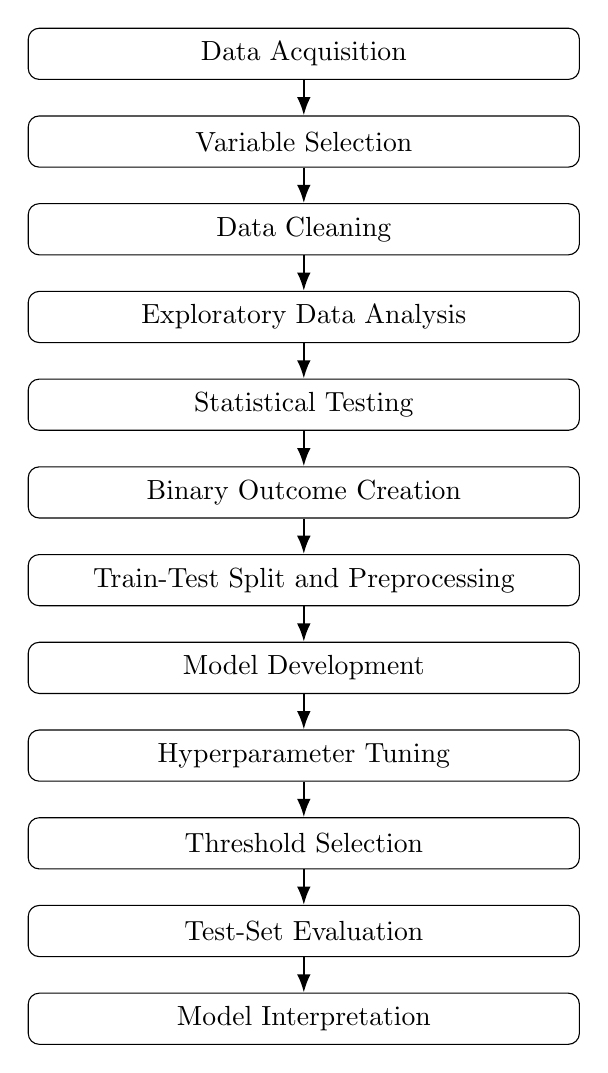
\begin{tikzpicture}[
    node distance=0.45cm,
    box/.style={
        rectangle,
        draw,
        rounded corners,
        align=center,
        minimum width=7cm,
        minimum height=0.65cm
    },
    arrow/.style={
        -{Latex},
        thick
    }
]

\node[box] (data) {Data Acquisition};
\node[box, below=of data] (variables) {Variable Selection};
\node[box, below=of variables] (cleaning) {Data Cleaning};
\node[box, below=of cleaning] (eda) {Exploratory Data Analysis};
\node[box, below=of eda] (testing) {Statistical Testing};
\node[box, below=of testing] (outcome) {Binary Outcome Creation};
\node[box, below=of outcome] (split) {Train-Test Split and Preprocessing};
\node[box, below=of split] (models) {Model Development};
\node[box, below=of models] (tuning) {Hyperparameter Tuning};
\node[box, below=of tuning] (threshold) {Threshold Selection};
\node[box, below=of threshold] (evaluation) {Test-Set Evaluation};
\node[box, below=of evaluation] (interpretation) {Model Interpretation};

\draw[arrow] (data) -- (variables);
\draw[arrow] (variables) -- (cleaning);
\draw[arrow] (cleaning) -- (eda);
\draw[arrow] (eda) -- (testing);
\draw[arrow] (testing) -- (outcome);
\draw[arrow] (outcome) -- (split);
\draw[arrow] (split) -- (models);
\draw[arrow] (models) -- (tuning);
\draw[arrow] (tuning) -- (threshold);
\draw[arrow] (threshold) -- (evaluation);
\draw[arrow] (evaluation) -- (interpretation);

\end{tikzpicture}

\caption{Overall Workflow of the Data Analysis and Predictive Modeling Process}
\label{fig:project_workflow}
\end{figure}

\section{Predictive Modeling Results}

\subsection{Modeling Sample and Class Distribution}

After applying the final data-cleaning criteria, the predictive modeling dataset contained 52,543 women. Of these respondents, 3,315 were classified as having low life satisfaction, while 49,228 were included in the comparison group.

As shown in Table~\ref{tab:target_distribution}, approximately 6.31\% of respondents reported low life satisfaction, while 93.69\% did not report low life satisfaction. This indicates that the outcome variable was highly imbalanced.

\begin{table}[H]
\centering
\caption{Class Distribution in the Final Modeling Sample}
\label{tab:target_distribution}
\begin{tabular}{lrr}
\hline
\textbf{Outcome Group} &
\textbf{Number of Respondents} &
\textbf{Percentage} \\
\hline
No Low Life Satisfaction & 49,228 & 93.69\% \\
Low Life Satisfaction & 3,315 & 6.31\% \\
\hline
Total & 52,543 & 100.00\% \\
\hline
\end{tabular}
\end{table}

A stratified 80--20 train-test split was used to maintain a similar proportion of low-life-satisfaction cases in both datasets. The training set contained 42,034 respondents, while the test set contained 10,509 respondents. The training data were used for model fitting, hyperparameter tuning, cross-validation, and threshold selection. The held-out test data were used only for final model evaluation.

The class imbalance was important when interpreting model performance. A model could achieve high accuracy by predicting that almost all respondents belonged to the majority group, while still failing to identify women with low life satisfaction. Therefore, model performance was evaluated using several measures in addition to accuracy.

\subsection{Hyperparameter Tuning Results}

Hyperparameter tuning was conducted for the Decision Tree and Random Forest models using stratified three-fold cross-validation. Average precision, also reported as PR-AUC, was used as the scoring measure because the low-life-satisfaction group represented a small proportion of the sample.

Table~\ref{tab:tuning_results} presents the best parameter combinations identified during cross-validation.

\begin{table}[H]
\centering
\caption{Selected Hyperparameters for the Tuned Models}
\label{tab:tuning_results}
\small
\begin{tabular}{p{3.4cm}p{8.5cm}r}
\hline
\textbf{Model} &
\textbf{Selected Parameters} &
\textbf{CV PR-AUC} \\
\hline
Tuned Decision Tree &
Maximum depth = 8; minimum samples per leaf = 250;
minimum samples required to split = 50 &
0.185 \\
\hline
Tuned Random Forest &
Number of trees = 200; maximum depth = 5;
minimum samples per leaf = 25; minimum samples required
to split = 250; maximum features = square root &
0.205 \\
\hline
\end{tabular}
\end{table}

The tuned Random Forest achieved a higher cross-validation PR-AUC than the tuned Decision Tree. However, the final value of a tuned model depends on how well it performs on the held-out test data rather than only on its cross-validation score.

\subsection{Model Performance at the Default Threshold}

All models were first evaluated using the standard probability threshold of 0.50. Table~\ref{tab:model_performance} presents the held-out test results.

\begin{table}[H]
\centering
\caption{Model Performance on the Held-Out Test Set at the Default Threshold}
\label{tab:model_performance}
\scriptsize
\resizebox{\textwidth}{!}{
\begin{tabular}{lrrrrrrrr}
\hline
\textbf{Model} &
\textbf{Accuracy} &
\textbf{Precision} &
\textbf{Recall} &
\textbf{F1} &
\textbf{Weighted F1} &
\textbf{Balanced Acc.} &
\textbf{ROC-AUC} &
\textbf{PR-AUC} \\
\hline
Baseline Model          & 0.937 & 0.000 & 0.000 & 0.000 & 0.906 & 0.500 & 0.500 & 0.063 \\
Logistic Regression     & 0.686 & 0.123 & 0.650 & 0.207 & 0.766 & 0.669 & 0.731 & 0.197 \\
Decision Tree           & 0.695 & 0.123 & 0.627 & 0.206 & 0.773 & 0.664 & 0.717 & 0.164 \\
Tuned Decision Tree     & 0.688 & 0.121 & 0.627 & 0.203 & 0.768 & 0.660 & 0.723 & 0.185 \\
Random Forest           & 0.677 & 0.121 & 0.661 & 0.205 & 0.760 & 0.669 & 0.733 & 0.201 \\
Tuned Random Forest     & 0.636 & 0.112 & 0.692 & 0.193 & 0.729 & 0.662 & 0.731 & 0.201 \\
Gradient Boosting       & 0.685 & 0.122 & 0.643 & 0.205 & 0.766 & 0.665 & 0.733 & 0.204 \\
\hline
\end{tabular}
}
\end{table}

The baseline model achieved an accuracy of 0.937 because it predicted the majority class for every respondent. However, its precision, recall, and F1-score for low life satisfaction were all zero. Therefore, the baseline model did not identify any women in the low-life-satisfaction group.

All non-baseline models identified substantially more low-life-satisfaction cases. At the default threshold, recall ranged from 0.627 for the Decision Tree models to 0.692 for the Tuned Random Forest. This means that the models identified approximately 63\% to 69\% of the respondents with low life satisfaction.

However, precision was low across the models, ranging from 0.112 to 0.123. Therefore, many respondents predicted to have low life satisfaction were false positives. This reflects the difficulty of predicting a relatively uncommon outcome.

ROC-AUC values ranged from 0.717 to 0.733 among the non-baseline models, indicating moderate ability to rank respondents according to their likelihood of low life satisfaction. Gradient Boosting and the standard Random Forest achieved the highest ROC-AUC of 0.733.

Gradient Boosting achieved the highest PR-AUC at 0.204, followed by the standard and tuned Random Forest models at approximately 0.201 and Logistic Regression at 0.197. These values were higher than the baseline PR-AUC of 0.063. However, the differences among Logistic Regression, Random Forest, and Gradient Boosting were small.

The more complex models therefore did not produce a large improvement over Logistic Regression. This supports the continued use of Logistic Regression as an important model because it provides similar predictive performance with more direct interpretation.

\subsection{ROC and Precision-Recall Analysis}

The ROC curves for the six non-baseline models are presented in Figure~\ref{fig:roc_models}. The curves were relatively close to one another, which is consistent with the small differences in ROC-AUC shown in Table~\ref{tab:model_performance}.

\begin{figure}[H]
\centering

\includegraphics[width=0.82\textwidth]
{./figures/roc_curve_models.png}
\caption{ROC Curve Comparison Across Classification Models}
\label{fig:roc_models}
\end{figure}

The precision-recall curves are shown in Figure~\ref{fig:pr_models}. Precision-recall analysis was particularly important because it focuses on the smaller positive class. Gradient Boosting had the highest PR-AUC, although its advantage over Random Forest and Logistic Regression was limited.

\begin{figure}[H]
\centering

\includegraphics[width=0.82\textwidth]
{figures/precision_recall_curve_models.png}
\caption{Precision-Recall Curve Comparison Across Classification Models}
\label{fig:pr_models}
\end{figure}

The ROC and precision-recall results suggest that the selected predictors contain meaningful information about low life satisfaction, but they do not completely separate the two outcome groups. This indicates moderate rather than strong predictive performance.

\subsection{Validation-Based Threshold Analysis}

The initial model comparison used the standard classification threshold of 0.50. However, this threshold may not provide the most useful balance between precision and recall when the outcome is highly imbalanced.

Thresholds were therefore selected for Logistic Regression, Tuned Random Forest, and Gradient Boosting using five-fold out-of-fold predictions from the training data. The threshold with the highest validation F1-score was selected for each model. The held-out test set was not used during threshold selection.

The selected thresholds were 0.65 for Logistic Regression, 0.65 for the Tuned Random Forest, and 0.70 for Gradient Boosting. Figure~\ref{fig:threshold_validation} shows how validation F1-score changed across the tested thresholds.

\begin{figure}[H]
\centering

\includegraphics[width=0.82\textwidth]
{./figures/threshold_tuning_validation_f1_scores.png}
\caption{Validation F1-Score Across Probability Thresholds}
\label{fig:threshold_validation}
\end{figure}

Table~\ref{tab:threshold_results} compares the default and validation-selected thresholds on the held-out test set.

\begin{table}[H]
\centering
\caption{Test-Set Results at Default and Validation-Selected Thresholds}
\label{tab:threshold_results}
\scriptsize
\resizebox{\textwidth}{!}{
\begin{tabular}{llrrrrrrr}
\hline
\textbf{Model} &
\textbf{Threshold Type} &
\textbf{Threshold} &
\textbf{Accuracy} &
\textbf{Precision} &
\textbf{Recall} &
\textbf{F1} &
\textbf{Weighted F1} &
\textbf{Balanced Acc.} \\
\hline
Logistic Regression &
Default & 0.50 & 0.686 & 0.123 & 0.650 & 0.207 & 0.767 & 0.669 \\

Logistic Regression &
Validation-selected & 0.65 & 0.860 & 0.193 & 0.385 & 0.257 & 0.881 & 0.638 \\

Tuned Random Forest &
Default & 0.50 & 0.636 & 0.112 & 0.692 & 0.193 & 0.729 & 0.662 \\

Tuned Random Forest &
Validation-selected & 0.65 & 0.891 & 0.225 & 0.297 & 0.256 & 0.898 & 0.614 \\

Gradient Boosting &
Default & 0.50 & 0.685 & 0.122 & 0.643 & 0.205 & 0.766 & 0.665 \\

Gradient Boosting &
Validation-selected & 0.70 & 0.887 & 0.225 & 0.320 & 0.264 & 0.897 & 0.623 \\
\hline
\end{tabular}
}
\end{table}

The validation-selected thresholds increased precision and F1-score for all three models. For example, the precision of Gradient Boosting increased from 0.122 to 0.225, while its F1-score increased from 0.205 to 0.264.

However, these improvements were accompanied by lower recall. Gradient Boosting recall decreased from 0.643 to 0.320, while Logistic Regression recall decreased from 0.650 to 0.385. The higher thresholds produced fewer false positives but also failed to identify more respondents with low life satisfaction.

Gradient Boosting achieved the highest threshold-selected test F1-score at 0.264, but the differences from Logistic Regression and Tuned Random Forest were small. Therefore, the validation-selected threshold should not be considered better for every purpose. The preferred threshold depends on whether the main priority is identifying more low-life-satisfaction cases or reducing false-positive predictions.

ROC-AUC and PR-AUC did not change when the classification threshold changed because these measures were calculated using the predicted probabilities across a range of possible thresholds.

\subsection{Logistic Regression Interpretation}

A separate reference-coded Logistic Regression model was fitted to support interpretation. One category from each categorical predictor was treated as the reference group. The resulting coefficients were converted into odds ratios.

Table~\ref{tab:selected_odds_ratios} presents selected results for variables that showed clear relationships with low life satisfaction.

\begin{table}[H]
\centering
\caption{Selected Reference-Coded Logistic Regression Odds Ratios}
\label{tab:selected_odds_ratios}
\begin{tabular}{p{5.2cm}p{5.1cm}r}
\hline
\textbf{Predictor Category} &
\textbf{Reference Category} &
\textbf{Odds Ratio} \\
\hline
Severe food insecurity &
Food secure &
4.605 \\

At least some functional difficulty &
No functional difficulty &
3.124 \\

Moderate food insecurity &
Food secure &
2.401 \\

Marginal food insecurity &
Food secure &
1.542 \\

Highest household income category &
Lowest household income category &
0.692 \\
\hline
\end{tabular}
\end{table}

Severe food insecurity had the largest selected odds ratio. Holding the other modeled predictors constant, women experiencing severe food insecurity had approximately 4.6 times the predicted odds of low life satisfaction compared with food-secure women.

Women reporting at least some functional difficulty had approximately 3.1 times the predicted odds of low life satisfaction compared with women reporting no functional difficulty. Moderate and marginal food insecurity were also associated with higher predicted odds of low life satisfaction.

The highest household income category had an odds ratio below 1 compared with the lowest income category, indicating lower predicted odds of low life satisfaction among women in the highest income group.

These odds ratios should be interpreted cautiously. They were obtained from a class-weighted and regularized predictive model and represent associations within the analytical sample. They should not be interpreted as causal effects or as formal population-level estimates.

\subsection{Variable Importance Across Models}

Predictor importance was also examined across Logistic Regression, Decision Tree, Random Forest, and Gradient Boosting. Because the importance values produced by different model types are not directly comparable, predictor categories were first combined into their original variables. Each variable was then ranked within each model, and an average rank was calculated.

Figure~\ref{fig:importance_rank} presents the combined variable-importance ranking.

\begin{figure}[H]
\centering

\includegraphics[width=0.82\textwidth]
{figures/feature_importance_rank_score_comparison.png}
\caption{Variable Importance Ranking Across Models}
\label{fig:importance_rank}
\end{figure}

Functional difficulty was the most consistently important variable across the models, with an average rank of 1.25. Food security was ranked second, with an average rank of 1.75, followed by labour force status with an average rank of 3.75.

Household size, age, province, and household income also contributed to model predictions, although their importance was less consistent across the different methods. Education, immigrant status, and visible minority status generally received lower importance rankings.

The model-based findings were generally consistent with the exploratory analysis. Both stages identified food security and functional difficulty as the two strongest factors, although their order differed slightly. Employment status and household income also appeared relevant, while education and province showed weaker or less consistent relationships.

Feature importance indicates how much a variable contributed to prediction within a particular model. It does not show that the variable caused low life satisfaction.

\subsection{Summary of Predictive Modeling Findings}

Several main findings emerged from the predictive modeling stage.

First, the high accuracy of the baseline model was misleading because it failed to identify any respondents with low life satisfaction. All non-baseline models improved the identification of the smaller positive class.

Second, predictive performance was moderate. ROC-AUC values were approximately 0.72 to 0.73, while PR-AUC values ranged from 0.164 to 0.204. Gradient Boosting produced the highest held-out PR-AUC, but its improvement over Random Forest and Logistic Regression was small.

Third, the default threshold produced relatively high recall but very low precision. Validation-selected thresholds improved precision and F1-score but reduced recall. This demonstrates that model performance depends partly on the purpose of classification and the relative importance placed on false positives and false negatives.

Fourth, more complex ensemble models did not substantially outperform Logistic Regression. Logistic Regression therefore remained useful because it provided competitive predictive performance together with clearer interpretation through reference-coded odds ratios.

Finally, functional difficulty, food security, and labour force status were the most consistently important predictors across the models. These results were generally consistent with the exploratory findings and suggest that health-related functioning and material conditions are important factors associated with low life satisfaction among women in the analytical sample.

The findings represent predictive associations rather than causal relationships. They should also be interpreted as results for the unweighted analytical sample rather than nationally representative estimates for all women in Canada.

\section{Discussion}

\subsection{Overview of the Main Findings}

This study examined factors associated with low life satisfaction among women using data from the 2022 Canadian Community Health Survey. The analysis combined exploratory data analysis, statistical testing, and predictive modeling to examine demographic, socioeconomic, employment-related, and health-related factors.

The exploratory and modeling results were generally consistent. Food security and functional difficulty showed the strongest relationships with low life satisfaction. Labour force status and household income were also important, while education, province, immigrant status, and visible minority status showed weaker or less consistent relationships.

The predictive models performed better than the majority-class baseline in identifying women with low life satisfaction. However, overall predictive performance was moderate. Gradient Boosting achieved the highest PR-AUC, but its improvement over Random Forest and Logistic Regression was small. This suggests that the selected predictors contained useful information, although they were not sufficient to clearly separate respondents with and without low life satisfaction.

The findings should be interpreted as associations and predictive patterns rather than causal relationships. Since the data were cross-sectional, it is not possible to determine whether the identified factors caused changes in life satisfaction or whether the relationships operated in the opposite direction.

\subsection{Food Security and Material Conditions}

Food security was one of the strongest factors identified in both the exploratory and predictive analyses. The descriptive results showed a clear increase in low life satisfaction as food insecurity became more severe. Women experiencing severe food insecurity reported much higher levels of low life satisfaction than food-secure women.

The reference-coded Logistic Regression results also showed that severe, moderate, and marginal food insecurity were associated with higher predicted odds of low life satisfaction compared with food security. Food security was also consistently ranked among the most important variables in the tree-based models.

These findings are consistent with previous research showing that food insecurity reflects broader financial hardship and material deprivation \citep{tarasuk2023}. Difficulty obtaining sufficient and appropriate food may be connected with uncertainty, stress, debt, housing pressures, and limited access to other basic resources. These conditions may influence how individuals evaluate their overall quality of life.

The results suggest that food insecurity is not only related to nutrition or physical health, but may also be an important indicator of subjective well-being. However, the relationship may involve several connected factors, including income, household structure, employment, and health status. Therefore, food security should not be interpreted as operating independently from other socioeconomic conditions.

\subsection{Functional Difficulty and Health-Related Factors}

Functional difficulty was the most consistently important variable across the predictive models. Women reporting at least some difficulty with seeing, hearing, walking, remembering, self-care, or communication were more likely to report low life satisfaction than women reporting no functional difficulty.

This finding was also supported by the exploratory analysis, where women with functional difficulties had substantially higher levels of low life satisfaction. The Logistic Regression model further showed higher predicted odds of low life satisfaction among women with functional difficulties after accounting for the other modeled variables.

Functional limitations may affect several areas of life. They can reduce independence, restrict participation in employment and social activities, increase the need for assistance, and make everyday tasks more difficult. These experiences may influence how respondents evaluate their overall quality of life.

The importance of functional difficulty is consistent with previous research linking health status and physical functioning with subjective well-being \citep{diener1984,denton2004}. However, because the data are cross-sectional, the direction of the relationship cannot be confirmed. Functional difficulties may contribute to lower life satisfaction, but lower well-being may also be connected with other health and social conditions that were not fully measured in the dataset.

Musculoskeletal chronic conditions were also associated with low life satisfaction, although their relationship was weaker than the relationship observed for functional difficulty. This may be because functional difficulty more directly reflects how health conditions affect daily activities, while the presence of a chronic condition does not necessarily indicate the same level of limitation for every respondent.

\subsection{Income and Employment-Related Factors}

Household income showed a clear relationship with life satisfaction during the exploratory analysis. Women in lower-income groups reported higher levels of low life satisfaction than women in the highest income group. The Logistic Regression results also indicated lower predicted odds of low life satisfaction among women in the highest income category compared with those in the lowest category.

These findings are consistent with previous research showing that income is associated with life evaluation and access to material resources \citep{kahneman2010}. Higher income may provide greater financial security and improved access to housing, food, transportation, healthcare, and recreational activities. Lower income may increase financial stress and reduce the ability to respond to unexpected expenses.

Labour force status was also an important predictor. Women who had not worked during the previous week generally reported higher levels of low life satisfaction than women who had worked. Employment may contribute to well-being through income, daily structure, social interaction, and a sense of purpose \citep{clark1994}.

However, employment status should be interpreted carefully. Some respondents may not have worked because of retirement, education, caregiving responsibilities, illness, disability, unemployment, or other reasons. These situations may have different relationships with life satisfaction. The grouped labour force variable used in the CCHS Public Use Microdata File did not allow all of these circumstances to be examined separately.

Employment does not necessarily lead to higher well-being in every situation. Poor-quality, insecure, or stressful employment may also negatively affect health and life satisfaction \citep{butterworth2011}. The current analysis included labour force status but did not include detailed measures of job quality, workplace control, job insecurity, or work-family conflict. These factors may help explain additional variation in life satisfaction.

\subsection{Demographic and Contextual Factors}

Education and province were statistically associated with low life satisfaction in the exploratory analysis, but their Cramer's V values were relatively small. They also showed lower or less consistent importance across the predictive models.

The weak relationship between education and low life satisfaction may indicate that education affects well-being indirectly through income, employment opportunities, health knowledge, or access to resources. Once these related variables were included in the models, education may have provided limited additional predictive information.

Differences in low life satisfaction across provinces were also modest. Provincial variation may reflect differences in economic conditions, public services, housing costs, population characteristics, and access to healthcare. However, province alone is a broad measure and may not capture important differences within provinces or between urban and rural communities.

Age, household size, immigrant status, and visible minority status also contributed less consistently across the models. This does not mean that these factors are unimportant to women's well-being. Their relationships may depend on interactions with income, employment, family responsibilities, health, discrimination, social support, or length of time in Canada.

The public-use dataset did not contain enough detail to examine all of these experiences. More focused research may be needed to understand how demographic and social identities interact with material and health-related conditions.

\subsection{Comparison of Exploratory and Modeling Findings}

The exploratory and predictive results were similar in several important ways. Both approaches identified food security and functional difficulty as the strongest factors associated with low life satisfaction. Household income and labour force status were also relevant, while education and province showed weaker relationships.

There was a small difference in the ordering of the most important variables. Food security had the largest Cramer's V during the exploratory analysis, while functional difficulty had the highest average importance rank across the predictive models.

This difference is reasonable because the two methods answer different questions. Cramer's V measures the strength of a bivariate relationship between one predictor and the outcome. Model-based importance reflects the contribution of a variable when several predictors are considered together. Predictor correlations, non-linear relationships, and interactions can therefore affect the importance ranking.

The consistency between the two stages strengthens the overall interpretation. The main findings were not based on only one statistical test or one predictive model. Instead, similar patterns appeared across descriptive results, Chi-square tests, Logistic Regression, and tree-based models.

\subsection{Model Performance and the Value of Interpretability}

All substantive models performed better than the majority-class baseline in identifying women with low life satisfaction. The baseline model achieved high accuracy but failed to identify any positive cases. This demonstrated that accuracy alone was not an appropriate measure for the imbalanced outcome.

The non-baseline models achieved moderate ROC-AUC and PR-AUC values. Their results suggest that the predictors contained meaningful information, but prediction remained difficult. Life satisfaction is likely influenced by many factors that were not included in the dataset, such as social support, relationship quality, caregiving burden, housing conditions, neighbourhood characteristics, discrimination, personal expectations, and recent life events.

Gradient Boosting achieved the highest PR-AUC, but its advantage over Random Forest and Logistic Regression was limited. The small difference suggests that greater model complexity did not produce a large improvement in predictive performance.

Logistic Regression remained valuable because it achieved competitive performance while providing more direct interpretation through odds ratios. This is important in a study where understanding associated factors is as important as classification performance.

The threshold analysis also showed that model performance depends on the purpose of prediction. Higher validation-selected thresholds improved precision and F1-score but reduced recall. Therefore, there was no single threshold that was best for every possible use.

A lower threshold may be preferred when identifying as many potentially at-risk respondents as possible is the main priority. A higher threshold may be preferred when reducing false-positive classifications is more important. Since this study was analytical rather than a clinical screening application, the threshold results were used mainly to demonstrate this trade-off.

\subsection{Implications of the Findings}

The results highlight the importance of considering both material conditions and health-related functioning when examining women's life satisfaction. Food insecurity, lower income, functional difficulty, and labour force status were more strongly associated with low life satisfaction than education or province.

These findings suggest that women's subjective well-being is connected with the conditions in which they live, work, and manage daily activities. Policies and programs aimed at improving well-being may therefore benefit from considering financial security, access to food, disability and functional support, and opportunities for appropriate employment.

The findings also show the value of combining exploratory analysis with predictive modeling. Exploratory analysis provided clear descriptions of group differences, while predictive models examined whether the variables remained useful when considered together.

The limited improvement from the ensemble methods also supports the use of interpretable models in social and public health research. When a simpler model performs similarly to a more complex model, the ability to clearly explain the findings may be more useful than a very small improvement in predictive performance.

These implications should be interpreted cautiously. The analysis did not evaluate specific programs or policy interventions, and it cannot show that changing one predictor would directly improve life satisfaction. The findings instead identify areas that may be useful for further research and more detailed population-level investigation.

\section{Conclusion}

This study examined demographic, socioeconomic, employment-related, and health-related factors associated with low life satisfaction among women in Canada using the 2022 Canadian Community Health Survey Public Use Microdata File. The analysis combined exploratory data analysis, statistical testing, and predictive modeling to provide both descriptive and model-based evidence.

The exploratory analysis was based on 52,884 women, while the final predictive modeling dataset contained 52,543 respondents after additional non-response categories were removed. Approximately 6.31\% of the modeling sample was classified as having low life satisfaction, which created a highly imbalanced classification problem.

The exploratory findings showed that food security and functional difficulty had the strongest associations with low life satisfaction. Women experiencing severe food insecurity reported substantially higher levels of low life satisfaction than food-secure women, while women with functional difficulties were more likely to report low life satisfaction than women without such difficulties. Household income and labour force status also showed meaningful relationships, while education and province had weaker associations.

The predictive modeling results were generally consistent with the exploratory findings. Functional difficulty, food security, and labour force status were the most consistently important predictors across the models. Household income, age, household size, and province also contributed to prediction, although their importance varied across methods.

All substantive models improved the identification of women with low life satisfaction compared with the majority-class baseline. Logistic Regression, Decision Tree, Random Forest, and Gradient Boosting achieved moderate predictive performance. Gradient Boosting produced the highest held-out PR-AUC, but its improvement over Logistic Regression and Random Forest was small. This suggests that more complex models did not provide a substantial predictive advantage over the simpler and more interpretable Logistic Regression model.

The threshold analysis showed an important trade-off between precision and recall. At the default threshold, the models identified a larger proportion of respondents with low life satisfaction but also produced many false-positive predictions. The validation-selected thresholds improved precision and F1-score but reduced recall. Therefore, the most appropriate threshold would depend on whether the main goal is to identify more potential cases or to reduce incorrect positive classifications.

The study contributes to the understanding of women's subjective well-being by examining several types of predictors within one analytical framework. It also demonstrates the value of combining descriptive analysis with interpretable and ensemble predictive models. The consistency of the findings across different methods provides support for the importance of material conditions and health-related functioning in relation to life satisfaction.

Several limitations should be considered. The CCHS is cross-sectional, and the findings cannot be used to establish causal relationships. The variables were self-reported, and some were grouped into broad categories in the public-use dataset. The binary outcome also simplified the original five-category life satisfaction measure by combining neutral responses with satisfied responses.

In addition, the analyses were based on unweighted data because no
suitable survey-weight variable was available in the processed datasets
used in this study. The results therefore describe associations within the analytical sample and should not be interpreted as nationally representative estimates for all women in Canada.

Future research could examine life satisfaction using longitudinal data to better understand how changes in income, food security, employment, and health are related to changes in well-being over time. Additional variables, including social support, caregiving responsibilities, housing conditions, job quality, relationship status, discrimination, and neighbourhood characteristics, may also improve understanding and prediction.

Future studies could also examine whether the identified relationships differ across age groups, income levels, immigrant groups, provinces, or other population subgroups. Where appropriate survey weights are available, weighted analyses could be used to produce more representative population estimates. External validation using another CCHS cycle or a different Canadian dataset would also help determine whether the predictive findings remain stable across samples and time periods.

Overall, the findings suggest that low life satisfaction among women is associated with a combination of material, employment-related, and health-related conditions. Food insecurity and functional difficulty were especially important across the exploratory and predictive analyses. Although the models provided moderate predictive performance, their main value was in identifying consistent factors associated with low life satisfaction and supporting a clearer understanding of women's well-being within the analytical sample.

\section{Project Repository}

The source code, notebooks, figures, tables, and project documentation associated with this study are available through the following GitHub repository:

\begin{center}
\url{https://github.com/Khushboosingh1988/MRP_CCHS_2022}
\end{center}

The repository contains the data preparation workflow, exploratory data analysis, predictive modeling notebooks, generated figures, statistical output tables, model evaluation results, and supporting project documentation.

The raw CCHS 2022 Public Use Microdata File is not included in the repository because of Statistics Canada data-use and licensing requirements. Instead, the repository includes documentation describing the data source, selected variables, project structure, and steps required to reproduce the analysis using an authorized copy of the dataset.

\bibliographystyle{apalike}
\bibliography{references}

\end{document}
